\chapter{La méthode Tomatis}

Nous  présentons ici la méthode Tomatis selon les cours et la formation acquise 
auprès d'Alfred Tomatis à Paris\footnote{Formation suivie dès 1995, Boulevard de Courcelles, Centre de l'écoute 
Tomatis à Paris; puis en 2009/11/13/15 avec V. Gas, V. Drouot et J.P. Granier, Elisabeth ...formateurs et consultants. Source: site internet officiel: \cite{tomatis.com}.}.


\section{Historique} 

Alfred Tomatis est né le 1er janvier 1920 et décédé le 25 décembre
2001. Il était docteur en médecine, spécialiste en oto-rhino-laryngologie,
connu mondialement pour ses travaux sur l'audition et la phonation.
Spécialisé particulièrement en neurophysiologie auditive, il a créé
une nouvelle discipline, l'audio-psycho-phonologie. Il a consacré
une grande partie de son activité professionnelle à étudier le relation
existante entre l'oreille et la voix, et par extension entre l'écoute
et la communication. Il s'agit de plus de cinquante ans de recherches
sur les fonctions de l'oreille. Ses découvertes furent établies au
laboratoire de physiologie de la Sorbonne et donnèrent lieu à des
communications à l'Académie des Sciences et à L'Académie de Médecine
de Paris en 1957 et 1960. Son \oe uvre représente plusieurs dizaines
de publications ainsi que treize ouvrages\footnote{Cf. la bibliographie.}.

\section{Définition de la méthode Tomatis} 
% ou définition de la méthode Tomatis?



La méthode Tomatis, créée par le sus-nommé, est une pédagogie et une
thérapie de l'écoute. Son outil est un appareil électronique appelé
\label{outil_oreille_electro}
Oreille Electronique avec  l'utilisation d'une technique particulière, la 
bascule, qui permet de créer une alternance entre deux conditions perceptives 
du même message sonore; passage soudain et imprévu de fréquences graves à des 
fréquences aiguës.

% ici il faut une référence et non un numéro qui 
%peut changer.
Il s'agit d'éducation\footnote{Cf. ch. 4.4.} \pdfmargincomment{Retrouver le passage} 
et / ou de rééducation. On parle\pdfcomment{Qui parle?} d'effet Tomatis qui permet au
cerveau d'améliorer naturellement \emph{l'interprétation du message
sensoriel.}

\subsection{L'audio-psycho-phonologie}

L'audio-psycho-phonologie aborde l'écoute comme
clé de décodage pour comprendre l'homme.

Tomatis était avant tout un clinicien à l'écoute de ses patients avec,
pour motivation première, l'application clinique de ses recherches.
Guidé par son intuition avec la faculté de remise en question des
théories appliquées ainsi que celle de créer des liens entres les
disciplines, il a pu élaborer un nouveau type de thérapie, dénommée
l'audio-psycho-phonologie. Elle regroupe trois disciplines, successivement,
l'audio (l'oreille) la psychologie et la phonologie (voix). La voix
dépend de l'oreille et sont, tous les deux, des outils de la communication
(psychologie). 
Tomatis accorde à l'oreille une place extrêmement importante. En soignant
des chanteurs à la voix déficiente, il a eu l'idée de leur tester
leur audition et a ainsi détecté des correspondances avec leurs difficultés
vocales. 

De là, il énonce les lois qui constituent ``l'effet Tomatis'' : 
\begin{itemize}
	\item La voix ne contient que ce que l'oreille entend.
	\item Si l'on modifie l'audition, la voix est immédiatement et 
inconsciemment
		modifiée.
	\item Il est possible de transformer la phonation par une stimulation 
auditive
		entretenue pendant un certain temps (loi de rémanence).
\end{itemize}

Elle agit simultanément sur trois fonctions essentielles de l'oreille
: l'audition, l'équilibre et la dynamisation.
\begin{itemize}
	\item Audition : lorsque l'on s'entend, on peut mieux se structurer.
	\item Réharmonisation : équilibre et coordination : le SNC (système 
nerveux
		central) est touché lors de l'écoute de musique par 
l'intermédiaire
		du vestibule. Il y a une action sur les troubles psychomoteurs, 
les
		réponses motrices deviennent plus fluides. Les 
dysfonctionnements
		correspondent à un état de non-équilibre neurophysiologiques 
plus
		ou moins prononçés. 
	\item Stimulation : dynamiser le cerveau par des fréquences spécifiques
		et par là-même le corps tout entier. Le son est nécessaire pour 
notre
		épanouissement personnel. L'oreille a besoin d'être stimulée 
pour
		énergétiser le cerveau et le corps. En privilégiant les 
musiques avec
		de grandes gerbes harmoniques (élevées, aiguës) on induit la 
stimulation
		de la formation réticulée.\footnote{Déf.: la formation 
réticulée est la partie centrale de la substance grise du tronc cérébral, 
constituée de nombreuses cellules nerveuses qui communiquent entre elles par de 
multiples jonctions appelées synapses.} En captant des milliers d'informations
		à chaque instant, l'oreille recharge le cerveau et lui permet 
d'être
		à l'écoute de soi et des autres. Pour qu'un cerveau 
``fonctionne'',
		il lui faut trois milliards de stimulations par seconde.
\end{itemize}



Cette méthode répond ainsi à plusieurs objectifs: éducatifs : apprentissages
des langues, de la musique ; rééducatifs : troubles psychologiques,
moteurs, troubles du langage ; et psychothérapeutiques : angoisse,
dépression. Cette interdisciplinarité, façon de regrouper les disciplines, se retrouve
aujourd'hui de plus en plus, comme en 
psycho-neuro-immunologie
(PNI) devenue actuellement discipline médicale de pointe.\footnote{La PNI étudie 
l'impact des événements psychiques sur le système immunitaire. Elle repose sur 
la mise en évidence d'interrelations entre le système
nerveux central, le système neuroendocrinien et le système immunitaire.
C'est une approche interdisciplinaire incorporant des données de la
psychologie, de la neuroscience, de la neurologie, dont l'endocrinologie
et l'immunologie. (entre autres) Source : Wikipédia, février 17.}
Celle-ci est due à une conception intégrative
de l'homme, puisqu'elle met en interaction toutes ses dimensions corporelles
et psychologiques dont 
les émotions et les cognitions.






\section{Conception différente de la physiologie auditive}

Tomatis  s'oppose sur plusieurs points à G. Békésy\footnote{Georg Békésy, prix 
Nobel de physiologie 1961.} au sujet de la
physiologie auditive : 
\begin{itemize}
	\item l'oreille moyenne et son rôle de transmetteur 
	\item l'analyse fréquentielle au niveau de la cochlée
\end{itemize}

Son originalité réside dans sa conception de la transmission du son
au niveau de l'oreille interne. 

\subsection{Un organe actif}

Il propose une nouvelle compréhension de l'oreille, celle-ci étant,
à son regard, un organe \emph{actif} % j'ai souligné
dans le sens suivant :
\begin{itemize}
	\item L'oreille moyenne, grâce aux muscles de l'étrier et du marteau, 
fait
		un travail de visée en ciblant les sons à écouter : le tympan 
se tend
		pour se mettre en résonance avec les sons à percevoir.
	\item Il fait aussi un autre travail qui est celui de sélectionner des 
sons
		pour se protéger : la tension tympanique se détend pour amortir 
l'intensité
		sonore qui inonde l'oreille interne. 
\end{itemize}

\subsection{Conception classique: un organe passif}

Selon la conception de G. Békésy,
l'oreille ne sert qu'à transmettre les sons de manière passive
comme peut le faire un micro. 
Le rôle des osselets se limite à la transmission du
son. 

\begin{figure}
	\centering
	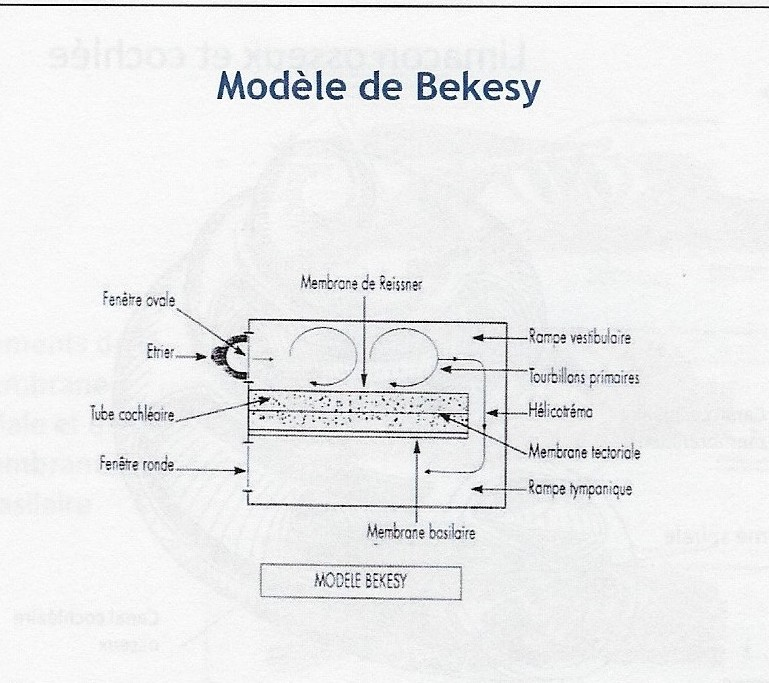
\includegraphics[width=0.7\linewidth]{images/Cochleederoule_bas.jpg}
	\caption[Modèle de Békésy]{Modèle de Békésy}
	\label{fig:cochleederoulebas}
\end{figure}

Comme déjà décrit plus haut,\footnote{Ch.2.4} les sons font vibrer le tympan 
qui,
étant attaché au marteau, répercute ces ondes acoustiques en mouvements 
mécaniques via les osselets. L'étrier transmet ensuite ces mouvements à 
l'oreille interne en jouant comme un piston au niveau de la fenêtre
ovale. L'information acoustique est alors transmise sous forme d'ondes
liquidiennes ou encore de tourbillons. Les tourbillons sont analysés (amplitude 
et vitesse) en termes de fréquences et de volume par les
cellules ciliées qui tapissent l'oreille interne.

\subsection{Conception de Tomatis}

Selon Tomatis, cette théorie a de nombreuses incohérences. L'une
d'entre elles serait que cette démonstration ne marche qu'avec un
\emph{son pur}\footnote{Un son pur est constitué d'une unique fréquence ou 
onde.}.
Or, les sons purs n'existent pas dans la nature, car ils sont, au
contraire, complexes et formés d'une multitude de fréquences et d'intensités
variées. Et cette complexité ne peut pas être transmise sans perte
et instantanément par des mouvements mécaniques et retransformée en
tourbillons. De plus, il y a un espace d'un millimètre entre l'enclume et 
l'étrier,
microscopique à l'\oe il nu mais  inexplicable sur le plan de la
physique pure.%
\footnote{Conférence au IIème Congrès International d'Audio-Psycho-Phonologie
Paris 1972:  \emph{Nouvelles théories sur la physiologie auditive}.}.

\begin{figure}
	\centering
	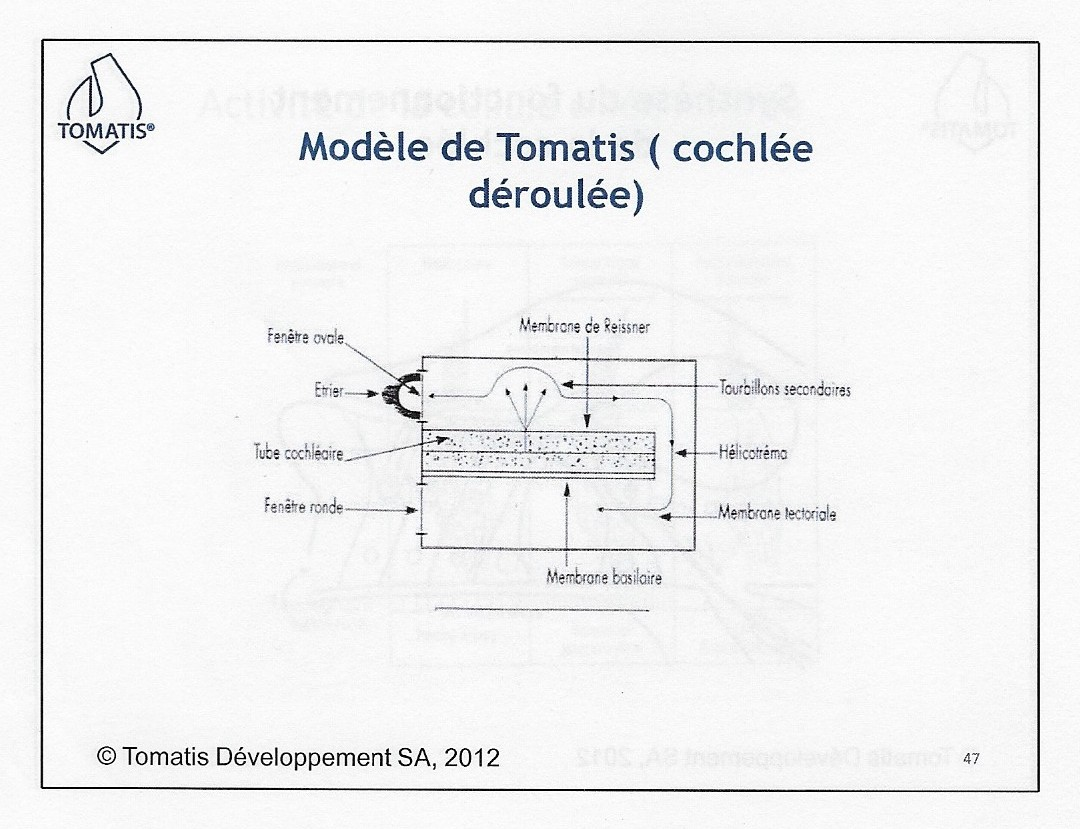
\includegraphics[width=0.7\linewidth]{images/Cochleederoule_haut.jpg}
	\caption[Cochlée selon Tomatis]{Cochlée selon Tomatis}
	\label{fig:cochleederoulehaut}
\end{figure}


On peut imaginer que le son passe
partout, par les ligaments de jonction des osselets ou les espaces
inter-ossiculaires mais % osseux?
ce n'était pas scientifiquement prouvable lors d'une de ses conférences
en 1972. L'est-il à l'heure actuelle? pas à notre connaissance. 

Nous allons aborder la conduction osseuse qui pourrait nous aider
dans cette compréhension.

\subsubsection{La conduction osseuse}

Lorsque l'on fait l'expérience de se
boucher les oreilles et de parler normalement, on se rend compte que
notre voix se propage principalement par les os de la tête. Comment
expliquer que l'on perçoive parfaitement bien les sons par conduction
osseuse en mettant un vibrateur conducteur de son sur la boîte crânienne et ce, 
même si l'oreille moyenne est abîmée (tympan percé, osselets non fonctionnels)?
Effectivement, selon le site oreillemudry.ch,\footnote{oreillemudry.ch}, 
le son stimule l'oreille de deux manières : par voie aérienne en transitant
par les trois parties de l'oreille et par voie osseuse en stimulant
directement l'oreille interne par vibrations des structures osseuses
qui l'entourent. On y relève l'importance de la voie osseuse
mais ne signale aucun nouvel élément dans la transmission
fréquentielle que celle dite classique, évoquée plus haut.

\subsubsection{Physiologie de l'audition selon Tomatis}

D'après Tomatis, les sons arrivent bien par le canal auditif
jusqu'au tympan. L'onde acoustique excite la membrane tympanique et
par voie de conséquence, l'os de la caisse du tympan. 
A l'instar d'une
peau de tambour qui fait chanter le bois auquel elle est attachée,
c'est toute la boîte crânienne qui inondée de sons et en particulier
l'oreille interne. Celle-ci, de par sa grande densité, capte les sons
et résonne comme du cristal\footnote{La transmission du son par l'os est de 
5000 $m/s$.}.

Les fréquences qui forment les sons vont ainsi exciter les cellules
ciliées qui tapissent la cochlée, tel un piano enroulé.

\paragraph{L'analyse multifréquentielle ne se pose plus}  
avec sa théorie: chaque fréquence se dirige instantanément et
naturellement vers la cellule ciliée qui lui correspond. 
C'est grâce à la forme particulière du limaçon qu'il y a un tri fréquentiel 
instantané.
Le son de fréquence identique s'installe toujours au même endroit, sur une 
ligne isofréquentielle, qui est une tranche perpendiculaire à l'axe.


\paragraph{Le rôle des tourbillons est de s'adapter aux bruits}
et non de transmettre les sons.
Lorsque l'intensité des sons aug\-men\-te,
l'ex\-ci\-ta\-tion des cellules ciliées provoque des perturbations liquidiennes
dans l'oreille interne, c'est-à-dire des tourbillons. Ceux-ci se propagent
et sont amortis par l'étrier. Si les sons atteignent une intensité
dangereuse pour les cellules ciliées, l'étrier réagit fortement et
entraîne une réaction du marteau qui modifie la tension du tympan.
A son tour, le tympan, relâché, amortit le volume sonore transmis
à l'oreille interne, comme la paupière qui se ferme quand la lumière
est trop intense.


\begin{quotation}
	Le tympan se met dans un certain état de tension pour jouer le
	rôle d'un diapason qui fait vibrer toute la boîte crânienne
	par l'intermédiaire du \emph{sulcus tympani}. 
	\emph{C'est toute la boîte crânienne qui vibre et qui transmet le son à 
la vésicule labyrinthique et non à la chaîne ossiculaire que l'on a l'habitude 
de considérer comme le véhicule du son.} La chaîne ossiculaire est un ensemble 
qui
	joue le rôle d'adaptateur, de régulateur et non de transmetteur. La
	conduction du son par l'air puis par l'os doit donc
	être étudiée d'une façon complémentaire afin que l'on
	puisse déterminer par la suite la posture d'écoute du sujet%
	\footnote{Entretien réalisé par B. Auriol avec Tomatis, Anvers 
1973.}.\pdfmargincomment{quel livre?}

\end{quotation}


Christine Petit note et relève par ces recherches le rôle important
et indéniable de la cochlée sur notre audition et spécifie qu'encore
à l'heure actuelle, il reste très mystérieux.

\nomenclature{cochlée}{Anatomie : organe de l'audition,appareil sensoriel, 
en forme de spirale, la cochlée, incluse dans l'os du rocher, 
forme le limaçon membraneux, se situe dans l'oreille interne et 
permet de déceler des sons extrêmement faibles, de discréminer des fréquences
et de masquer des sons faibles par des sons forts.}
<<\,C'est une sorte de minuscule appareil électroacoustique capable
de discréminer des sons extrêmement faibles, capable de \emph{masquer
les sons faibles par des sons forts}, pouvant \emph{distordre les
sons,} et en conséquent, \emph{capable d'élaborer un traitement extrêmement
sophistiqué des sons}%
% OGA: référence stp. Salters et Gaullier ont publié? émission?
\footnote{Christine Petit, titulaire de la chaire Génétique et
physiologie cellulaire au Collège de France, entretien en novembre 2012, 
réalisé par Laurent Salters et Vincent Gaullier, 
Look at science : le système sensoriel auditif confirme 
lors d'un entretien réalisé en 2012 le rôle indéniable de la cochlée.\,>>}.



 \paragraph{Etudes scientifiques et cliniques}
 Au fil des années, de nombreuses études scientifiques et cliniques
 ont été faites. Il est possible d'en trouver le contenu complet sur le site
internet officiel Tomatis : \emph{Tomatis Research and Publication}  
\footnote{www.tomatisassociation.org}.
 Nous citerons celle du Dr. med. Inge Flehming, neurologue et 
pédiatre\footnote{Dr. med. Inge Flehming,
	neurologue, neuropédiatre, texte publié en allemand
	en 1996, \emph{``Grundsatz-Gutachten zur Behandlungsmethode
		nach Prof. Tomatis''}. Voir 
\href{http://www.analytische-hoertherapie.de/uploads/tx\_templavoila/Grundsatzgu
tachten\_zur\_Behandlungsmethode\_nach\_Prof.\_Tomatis.pdf}{le site web.}}
 ainsi que celle notamment du Docteur Du Plessis sur l'effet
Tomatis sur l'anxiété en milieu scolaire et universitaire\footnote{Troubles 
psychologiques : Etude du Plessis (Université de Potchefstroon
- Afrique du Sud).}  \footnote{Du même auteur, une autre étude démontre qu'après 14,3
mois le niveau d'an\-xié\-té avait continué à baisser fortement
pour le groupe Tomatis alors qu'aucun
changement n'apparaissait pour le groupe contrôle}%
\footnote{Du Plessis W. F. and Van Jaarsveld, P. E. (1988),
	``Audio-psycho-phonology : A comparative outcome study on anxious 
primary school pupils'',  Afr. Tydskr. Sielk. 1988,
	18 (4) 144--151. Du Plessis, W.F., Burger, S. (2001) [\ldots]
	\emph{A pilot study involving the Tomatis method.}, Sud Africa J. 
Psychol.}
 
L'effet d'une technique particulière employée avec l'Oreille Electronique
--- la bascule \label{bascule} électronique a pour objectif de stimuler le cerveau en lui 
permettant de capter plus facilement les sons.
Cette étude pilote du Dr. Carlos Escera
de l'Université de Barcelone en 2014, menée en collaboration avec le CNRS  a fait 
l'objet d'une validation
par un comité de lecture scientifique. %
\footnote{%
\href{http://tomatisassociation.org/scientific-validation-of-the-tomatis-effect-
eeg-recordings-of-sound-from-brainstem-to-cerebral-cortex-encoding-university-of
-barcelona-2014/}{tomatisassociation.org}.}  \label{bascule}{.\footnote{La bascule permet 
de créer une alternance entre deux 
conditions perceptives du même message sonore: passage soudain et imprévu de 
fréquences graves à des fréquences aigües.}







 En conclusion, selon Pierre Lane, journaliste de l'é\-mi\-s\-sion Envoyé 
spécial%
\autocite{tomatis_methode_1991}, Tomatis
a inventé une méthode qui est très critiquée mais qui a donné des
résultats. Elle ouvre l'oreille par des procédés mécaniques pour atteindre
des domaines spécialisés, que ce soit en médecine, en psychologie,
en ostéopathie. C'est un outil proposé
en complément de la pratique de nombreux spécialistes. 

\section{Technique de travail sous ``Oreille électronique''}

Dès 1952, comme preuve et application des trois lois qu'il avait énoncées,
Tomatis a concentré ses efforts de recherche sur la mise au point
d'un appareil susceptible de modifier la manière d'entendre et, par
voie de conséquence, la façon de parler d'un sujet. Par cet appareil,
le but était d'obliger l'oreille à utiliser un mode d'accommodation
déterminant une manière d'entendre typique et entraînant le geste
vocal correspondant.

L'oreille va donc se tendre
vers l'information qui lui arrive.  Et si on met l'Oreille électronique en 
parallèle avec une
oreille qui ne rentre pas dans cette dynamique, elle va l'entraîner.
Elle sert à faire faire une gymnastique bien précise ou un jeu de
contractions.

L'adaptation de l'oreille moyenne se fait par le jeu des contractions
du muscle du marteau et du muscle de l'étrier.
\begin{itemize}
\item Le muscle du marteau agit sur la convexité imposée au tympan, qui
se comporte alors comme une lentille acoustique, sorte de cristallin
auditif.
\item Le muscle de l'étrier régule le jeu de l'oreille interne, qui sait,
à la manière d'un prisme, étaler la gamme des sons en spectre acoustique.
\end{itemize}

L'Oreille Electronique impose ce jeu à l'oreille.


Dans le but de faire faire cette gymnastique microscopique aux muscles
de l'oreille, ces musiques peuvent être préparées avec un jeu de bascule%
\footnote{Cf. explication au point \ref{bascule}, p. \pageref{bascule}.} 
qui alterne le passage des basses aux hautes
fréquences; elles peuvent aussi l'être avec un certain pourcentage
de filtrages qui va varier et s'ajuster selon la personne
et le résultat des tests d'écoute. Pour stimuler le désir d'écoute
du patient, il est aussi possible de préparer des musiques avec une
technique particulière, dénommée \emph{retard}, agissant sur le muscle de
l'étrier, c'est-à-dire sur la conduction osseuse. Une autre technique
est celle de la \emph{précession}, qui aidera à viser et décoder les messages,
en agissant sur le tympan, c'est-à-dire sur la conduction aérienne. 
Le travail sous Oreille Electronique va tendre
à faire revenir le sujet à un état d'équilibre : ainsi les progrès
observés se maintiennent et ne sont donc pas dûs à un conditionnement.
Le processus d'évolution a été rétabli dans sa normalité.

\section{Travail ``passif'' et ``actif'' sous Oreille Electronique}
\label{travail_sous_oreille_electronique}

\subsection{Technique dans le travail passif et actif}

La façon générale de procéder est:
\begin{itemize}
\item  l'alternance d'écoute de musiques;
\item le travail actif avec la voix;
\item des tests d'écoute;
\item des pauses.
\end{itemize}

Avant les séances : un test d'écoute, focus sur l'audition avec un
graphique.

Après les séances : le même test, avec visualisation d' une évolution
ou d'une transformation de l'écoute du patient : un changement sera
visible ou ne le sera pas.

\subsubsection{Dans le travail passif}

\begin{description}
\item [{1\iere session}] de 25 à 30h d'écoute : le patient écoute
deux heures de musique par jour pendant 13 à 15 jours consécutifs;
un deuxième test à la fin de ce travail; ensuite, une pause pendant
4 à 6 semaines.
\item [{2\ieme session}] de 25 à 30h d'écoute : 3ieme Test, à nouveau
deux heures d'écoute pendant 13 jours à 15 jours; puis 4\ieme test,
suivi d'une pause d'une durée de 4 à 8 semaines.
\item [{3\ieme session}] : la même façon de procéder que les deux
autres. 
\end{description}
Le choix et le traitement des musiques peuvent être très différents
selon le patient et sa pathologie.

But du travail passif : \emph{ouverture} de l'oreille
aux sons : sensibiliser à certains sons avec l'objectif de réintégrer
des fréquences perdues ou annihilées inconsciemment ou volontairement. 

Cette technique de travail se sert du son pour provoquer un résultat
physiologique. Elle dérange les habitudes d'écoute pour faire agir
et ré-agir le patient. Cette phase est parfois trop pertubatrice et fait 
l'objet de rejet 
par le patient.

\subparagraph{Dans le travail actif :}

Après avoir été stimulé et ouvert aux sons environnants, le patient
est amené par le thérapeute à travailler sa voix. On cible un travail
actif de la voix à l'aide des écouteurs spécifiques de la méthode
car la correction de la voix y est instantanée et instaure les bons
réflexes de la boucle audio-vocale. C'est un processus naturel par
lequel l'individu assimile et analyse l'information sonore qu'il reçoit
et ajuste en retour l'information sonore qu'il émet. Le patient va
commencer à s'en servir ``à volonté'', c'est-à-dire d'ajuster et
d'analyser ce va-et-vient permanent entre l'écoute et l'émission vocale
afin de créer une forme de réflexes sur lesquels il peut ``s'asseoir''. 

Cette phase de la thérapie est importante et parfois très délicate
pour le patient. C'est une phase que nous nommerions spécifique au domaine de 
la musicothérapie.  Accepter d'entendre sa propre voix n'est pas toujours
simple et l'encadrement et le soutien sont nécessaires pour permettre
au patient de franchir cette étape. Lorsqu'elle se passe bien, il
y a en quelque sorte réintégration de la voix dans le corps. Le patient
apprend à créer lui-même cette boucle phonatoire sur laquelle il va
pouvoir se reposer, se ressourcer, se régénérer pour être totalement
autonome au bout de sa restructuration : une reprise en main qui va
lui permettre d'``être et de se sentir auteur de sa propre vie''. 

\enquote{\emph{L'émission vocale confirme et reconfirme à chaque
fois le sujet dans son intégrité et son identité.}}%
\autocite[Tomatis en fait une description précise dans la troisième partie de
son livre, pp. 185--301]{tomatis:loreille}



% en biblio stp?
vocal sur le point d'être réalisé\footnote{Jean-Pierre Granier, Tomatis 
Développement,\emph{Conférence Paris lors de la Convention du 13 mai 2012}, 13.5.2012.}.
